\chapter{德西特視界與宇宙學機率}

\lectureoverview{視界不只是因果邊界。對靜止觀測者而言，視界是一個熱系統：在距視界固有距離 \(\rho\) 處放置溫度計，讀數的溫度量級為 \(1/(2\pi\rho)\)；引力紅移則使遠處觀測者看到的輻射冷得多。我們將把黑洞帶來的這項認識應用到德西特空間，推導固定的視界半徑 \(H^{-1}\)，並寫出觀測者靜態區的度規。講座後半將循著熱力學，探討它令人不安的後果：有限的德西特熵、龐加萊復現、波茲曼大腦、永恆暴脹，以及測度問題。最後的討論將弦理論中精確的超對稱結構，與可能描述我們世界、但目前仍未知的理論架構區分開來。}

\section{視界為何是熱的}

正式講座開始前，我們先從一個決定今晚討論方向的問題談起。

\begin{classroomqa}
\audiencequestion{宇宙視界中沒有黑洞。那麼，視界怎麼還會是熱的？其機制是什麼？\lecturetimestamp{00:00:17}}
\lecturerresponse{其機制與黑洞視界相同。關鍵在於操作上的問題：在視界附近放置的溫度計會測得什麼？又會有哪些輻射到達遠處的觀測者？}
\end{classroomqa}

第一個實驗是在局部進行。將溫度計固定在距任意光滑、非極端視界的固有距離 \(\rho\) 處。足夠靠近視界時，幾何具有普適的 Rindler 形式，溫度計的讀數為
\begin{equation}
T_{\rm local}(\rho)\simeq \frac{1}{2\pi\rho}
\label{eq:l09-local-temperature}
\end{equation}
這裡採用 \(\hbar=c=k_B=1\) 的單位制。代回常數後，得到
\begin{equation}
k_B T_{\rm local}(\rho)\simeq \frac{\hbar c}{2\pi\rho}.
\end{equation}
當 \(\rho\to0\) 時，溫度發散；但這不表示自由下落的觀測者會遇上一座普通的物質火爐。這是對一位始終停留在視界外、因此必須持續猛烈加速的觀測者而言的溫度。

開場的對話也區分了三個容易混淆的概念：能量、溫度和熵。

\begin{classroomqa}
\audiencequestion{如果把光子送進黑洞，我們測得的熵還會相同嗎？還是只有能量會改變？\lecturetimestamp{00:01:22}}
\lecturerresponse{光子一旦落到視界後方而無法被觀測，額外的資訊就被隱藏了。用這裡採用的簡化位元說法，一個光子可以隱藏一個額外位元，因而增加熵。能量、溫度和熵彼此相關，但不能互相替代。}
\end{classroomqa}

\editorialnote{物理黑洞的熵變由熱力學關係 \(dS=dE/T_H\) 決定；並非不論光子的能量為何，每個光子都一律使熵增加一個位元。「一個位元」是講座採用的資訊理論理想化說法。}

近視界區域不斷發射並重新吸收高頻量子漲落。對靜止觀測者而言，視界使這些漲落呈現熱性。然而，這立刻引出一個疑問：如果該區域熱得沒有上限，為什麼遠處的觀測者沒有被能量高得沒有上限的光子閃瞎？

\section{紅移與霍金溫度}

即使我們站得很遠，普通的高溫牆壁仍會發出高頻輻射。視界則不同，因為從視界發出的輻射必須穿過引力紅移。光子的速度仍是 \(c\)；降低的是它的能量，
\begin{equation}
E=\hbar\omega,
\qquad
\omega_{\rm received}<\omega_{\rm emitted}.
\end{equation}
講座中用粉筆作的類比，只在這個程度上有用。拋出的石頭上升時會減速；光子則仍以光速前進，只是頻率和能量降低。

對 Schwarzschild 黑洞，無窮遠處的觀測者測得的溫度為
\begin{equation}
T_H=\frac{1}{8\pi M}
\label{eq:l09-hawking-natural}
\end{equation}
這裡採用 \(G_N=\hbar=c=k_B=1\) 的單位制。以一般單位表示則為
\begin{equation}
T_H=\frac{\hbar c^3}{8\pi G_N M k_B}.
\label{eq:l09-hawking-full}
\end{equation}

\begin{figure}[htbp]
\centering
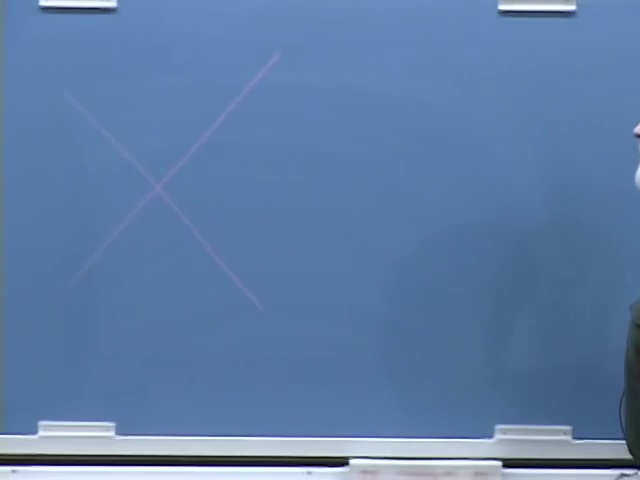
\includegraphics[width=0.68\textwidth]{lecture_09_figure_02.png}
\caption{自然單位制下的霍金溫度 \(T_H=1/(8\pi M)\)。}
\lectureframe{00:08:12}
\end{figure}

黑洞越大，溫度越低。講座透過反向追溯典型光子的路徑來說明這一點。熱光子的特徵能量為 \(E_\gamma\sim T_H\)。光子抵達無窮遠時的能量若約為 \(M^{-1}\)，那麼它從視界附近出發時的局域能量就大得多。對較大的黑洞而言，近視界區域到無窮遠處之間的紅移更強，因此到達無窮遠處的溫度較低。

\begin{classroomqa}
\audiencequestion{如果 Schwarzschild 時間在視界處凍結，我們是不是該追蹤最初落入、使黑洞形成的那個光子？\lecturetimestamp{00:04:19}}
\lecturerresponse{討論溫度時，應該追蹤向外發射的光子。它們從局域頻率極高的狀態出發，向外傳播時能量逐漸降低，最後以霍金輻射的形式抵達。最初落入的光子後來如何，則是另一個資訊問題。}
\end{classroomqa}

\section{普朗克層與拉伸視界}

方程式~\eqref{eq:l09-local-temperature}中的局域關係，在哪個範圍內可信？講座將普朗克長度視為半經典描述中有意義的最短距離。據此可想像一個薄層，大約位於數學視界外一個普朗克長度處，充滿普朗克尺度的漲落，並持續發射和吸收粒子。

大多數發射出的量子都無法逃逸。只有朝著非常狹窄的向外錐角傳播的量子，才不會落回視界。以一般角度發射的量子則會返回視界。出射與入射的激發彼此碰撞，產生粒子對和其他粒子；就這個意義而言，定態描述中包含一層極熱物質薄殼。

\begin{figure}[htbp]
\centering
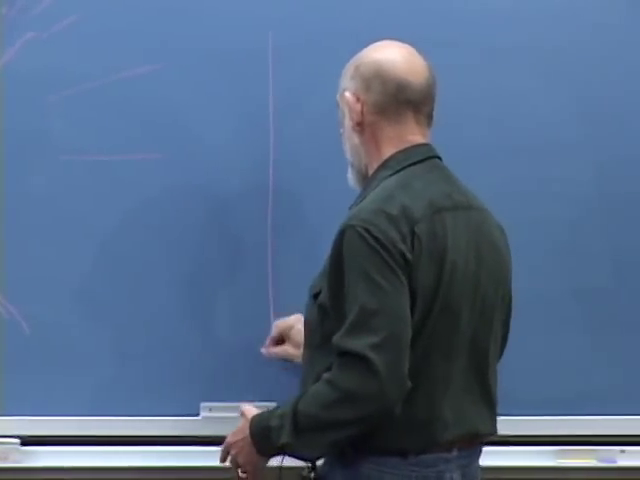
\includegraphics[width=0.74\textwidth]{lecture_09_figure_03.png}
\caption{近視界輻射的狹窄逃逸錐。局域發射的量子大多會返回視界。}
\lectureframe{00:11:38}
\end{figure}

從時空的角度來看，還有一種互補的圖像。在遠離視界之處，虛漲落可以示意性地表示為短暫的封閉迴圈：粒子—反粒子激發出現後便消失，來不及成為漸近態。在視界附近，漲落可以跨越因果邊界。對外部觀測者而言，位於外側的部分看起來像是視界發出、之後又重新吸收的粒子。只有極少部分會逃逸，成為霍金輻射。

\begin{classroomqa}
\audiencequestion{在外部圖示中，這種漲落是否從 \(t=-\infty\) 延伸到 \(t=+\infty\)？\lecturetimestamp{00:15:00}}
\lecturerresponse{精確的經典視界會導致這種看來奇異的描述。實際上，我們以拉伸視界取代它：在外部約一個普朗克長度處設置一道類時曲面。如此一來，發射和重新吸收便發生在有限的外部時間內。}
\end{classroomqa}

\begin{figure}[htbp]
\centering
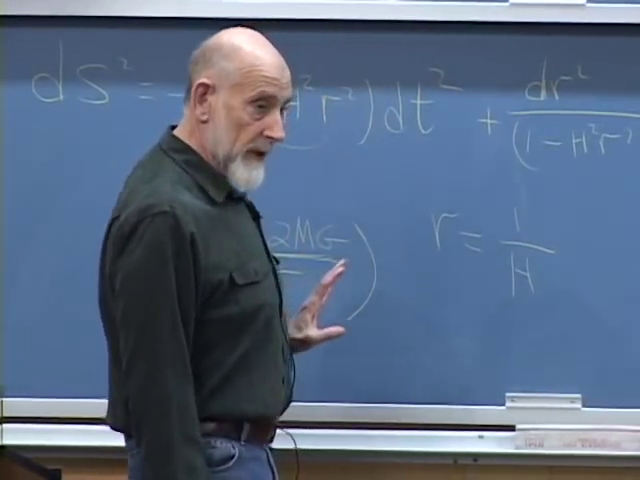
\includegraphics[width=0.72\textwidth]{lecture_09_figure_04.png}
\caption{經典視界，以及外部描述所採用的鄰近拉伸視界。}
\lectureframe{00:15:52}
\end{figure}

拉伸視界不是新的不變邊界，而是一個有效曲面，設在半經典幾何不再可靠的位置。物質和幾何本身的量子漲落，會在普朗克尺度上模糊精確的位置。這個做法將那種不確定性集中表現在一道曲面上，讓外部描述在此仍保持有限。

這個局域論證本身並不涉及視界究竟屬於黑洞，還是屬於加速膨脹的宇宙。這正是連結到德西特空間的橋梁。

\section{膨脹座標中的德西特空間}

正式講座從德西特時空的空間平坦切片開始，
\begin{equation}
ds^2=-dt^2+e^{2Ht}d\mathbf{x}^2,
\qquad
d\mathbf{x}^2=dx^2+dy^2+dz^2.
\label{eq:l09-flat-slicing}
\end{equation}
常數 \(H\) 是德西特膨脹率。度規中的因子為 \(e^{2Ht}\)，因為度規描述的是距離的平方；固定的座標間隔所對應的物理長度為
\begin{equation}
D(t)=e^{Ht}\lvert\Delta\mathbf{x}\rvert.
\end{equation}

\begin{figure}[htbp]
\centering
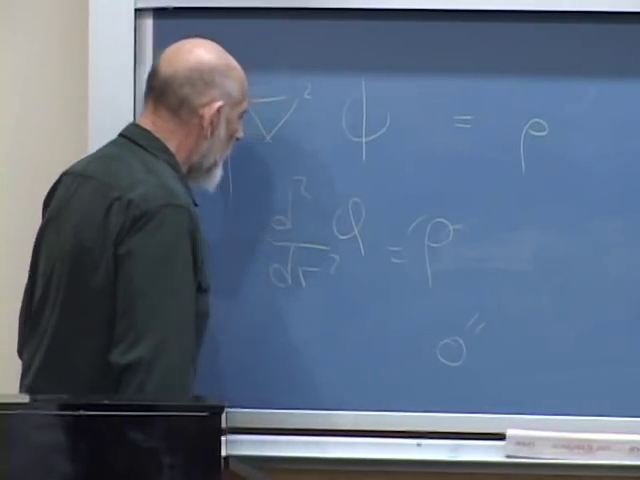
\includegraphics[width=0.78\textwidth]{lecture_09_figure_05.png}
\caption{平坦座標中呈指數膨脹的德西特度規。}
\lectureframe{00:18:50}
\end{figure}

這些座標清楚呈現了膨脹，但未來無窮遠仍在圖面上方無窮遠處。為了把它移到黑板上的有限位置，引入共形時間
\begin{equation}
\eta=-\frac{1}{H}e^{-Ht},
\qquad
-\infty<\eta<0.
\label{eq:l09-conformal-time}
\end{equation}
於是
\begin{equation}
dt=\frac{d\eta}{-H\eta},
\qquad
e^{Ht}=-\frac{1}{H\eta},
\end{equation}
方程式~\eqref{eq:l09-flat-slicing}便成為
\begin{equation}
ds^2=\frac{1}{H^2\eta^2}
\left(-d\eta^2+d\mathbf{x}^2\right).
\label{eq:l09-conformal-metric}
\end{equation}
當 \(t\to+\infty\) 時，\(\eta\to0^{-}\)。無限長的固有時間因此被壓縮到有限的水平線 \(\eta=0\)。

\editorialnote{黑板上的時間變換在書寫時修正了好幾次。方程式~\eqref{eq:l09-conformal-time}才是自洽的形式：早期宇宙時間對應到\(\eta\to-\infty\)，未來無窮遠則對應到\(\eta\to0^{-}\)。}

\begin{figure}[htbp]
\centering
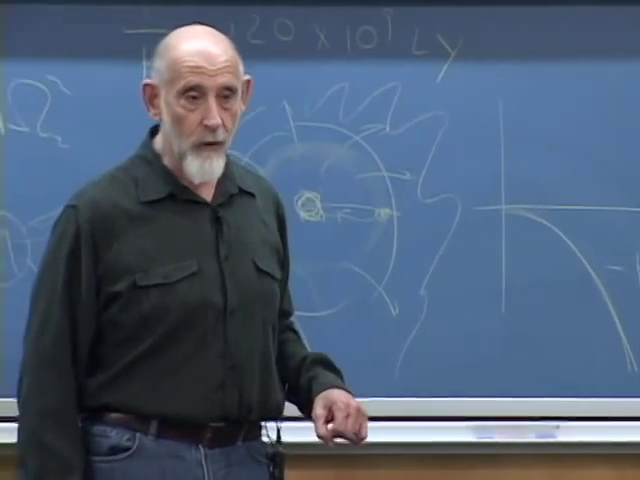
\includegraphics[width=0.82\textwidth]{lecture_09_figure_06.png}
\caption{共形時間變換與共形平坦度規。}
\lectureframe{00:21:24}
\end{figure}

共形因子同時乘在時間項和空間項上，因此不會改變零方向。對徑向光線而言，
\begin{equation}
ds^2=0
\quad\Longrightarrow\quad
-d\eta^2+dx^2=0
\quad\Longrightarrow\quad
\frac{dx}{d\eta}=\pm1.
\label{eq:l09-null-rays}
\end{equation}
所以光在共形圖中沿著 \(45^\circ\) 的方向傳播。這正是這種座標變換有用之處：因果上的可達範圍一目了然。

\section{單一觀測者的因果區域}

設想一位世界線延續無限固有時間的觀測者。在緊緻化的時空圖上，這條世界線終止於 \(\eta=0\) 上的一點。觀測者可能接收到的所有訊號，都位於該終點的後向光錐內。無論觀測者等待多久，光錐外的事件都不可能與他聯繫。

\begin{figure}[htbp]
\centering
\includegraphics[width=0.78\textwidth]{lecture_09_figure_07.png}
\caption{共形德西特座標中，觀測者的極限後向光錐。}
\lectureframe{00:24:38}
\end{figure}

另一位觀測者會有不同的光錐。兩人的可及區域彼此重疊，但都不涵蓋整個時空。接下來的論證將採取第一位觀測者的觀點，並把他的後向光錐稱為其因果區域。

圖上看來，這個區域朝未來逐漸縮小，但座標寬度不等於固有距離。在 \(\eta\) 為常數的切片上，位於 \(x=0\) 的觀測者與位於 \(x=\Delta x\) 的視界之間，物理距離的平方為
\begin{equation}
D^2=\frac{(\Delta x)^2}{H^2\eta^2}.
\label{eq:l09-horizon-distance-start}
\end{equation}
視界是一條 \(45^\circ\) 的零線，終止於 \(\eta=0\)，因此
\begin{equation}
\Delta x=\lvert\eta\rvert.
\end{equation}
代入後得到
\begin{equation}
D_{\rm hor}^2=\frac{1}{H^2},
\qquad
D_{\rm hor}=\frac{1}{H}.
\label{eq:l09-horizon-radius}
\end{equation}
座標間隔雖然縮小，共形因子卻恰好以相應比例增大。固有視界半徑維持不變。

\begin{figure}[htbp]
\centering
\includegraphics[width=0.80\textwidth]{lecture_09_figure_08.png}
\caption{黑板推導：將縮小的座標間隔換算為固定的固有距離 \(H^{-1}\)。}
\lectureframe{00:28:42}
\end{figure}

\section{靜態區}

視界半徑固定，表示可以採用適合中心觀測者的座標。講座未推導座標變換，而是直接寫下結果：
\begin{equation}
ds^2=
-\left(1-H^2r^2\right)d\tau^2
+\frac{dr^2}{1-H^2r^2}
+r^2d\Omega_2^2.
\label{eq:l09-static-patch}
\end{equation}
度規係數依賴 \(r\)，不依賴 \(\tau\)。這組座標涵蓋觀測者的靜態區：
\begin{equation}
0\le r<\frac{1}{H}.
\end{equation}

\begin{figure}[htbp]
\centering
\includegraphics[width=0.88\textwidth]{lecture_09_figure_09.png}
\caption{德西特靜態區度規，以及與 Schwarzschild 因子的比較。}
\lectureframe{00:34:22}
\end{figure}

它與 Schwarzschild 度規的相似之處一目了然：
\begin{equation}
f_{\rm dS}(r)=1-H^2r^2,
\qquad
f_{\rm Schw}(r)=1-\frac{2G_NM}{r}.
\end{equation}
兩種情況下，靜態座標中的視界都出現在 \(f(r)=0\) 處。對德西特空間而言，
\begin{equation}
1-H^2r^2=0
\quad\Longrightarrow\quad
r_H=H^{-1}.
\end{equation}
座標在此處呈現奇異性，就像 Schwarzschild 座標在黑洞視界處一樣。不過，整體幾何有一項重要差異：黑洞觀測者身在外部，向內看；德西特觀測者則身在內部，向外看。

\begin{classroomqa}
\audiencequestion{在指數膨脹的宇宙中，自由釋放的粒子會彼此遠離，幾何怎麼可能是靜態的？\lecturetimestamp{00:36:06}}
\lecturerresponse{靜態不表示每個粒子都保持不動，而是指度規係數和重複實驗的結果都不隨起始時間改變。現在釋放兩個粒子，它們會加速分離；稍後以相同方式重做實驗，粒子仍會有相同的運動。}
\end{classroomqa}

\begin{classroomqa}
\audiencequestion{這兩個彼此遠離的粒子會看到對方的光發生紅移嗎？\lecturetimestamp{00:38:34}}
\lecturerresponse{會。兩者間距持續增加，會造成相對紅移，即使適合觀測者的度規不隨時間改變。}
\end{classroomqa}

\section{從內部觀測到的溫度}

Schwarzschild 空間和德西特空間的近視界結構在局部是等價的。因此，德西特視界會發射並重新吸收熱量子。少數光子會向內傳播至中心觀測者，沿著靜態區的位勢向內傳播時能量逐漸降低。中心觀測者測得的 Gibbons---Hawking 溫度為
\begin{equation}
T_{\rm dS}=\frac{H}{2\pi}
\label{eq:l09-de-sitter-temperature}
\end{equation}
此處採用自然單位制。半徑 \(r\) 處的靜止溫度計，讀數則是經 Tolman 紅移後的溫度
\begin{equation}
T_{\rm local}(r)=
\frac{T_{\rm dS}}{\sqrt{1-H^2r^2}},
\label{eq:l09-tolman}
\end{equation}
當 \(r\to H^{-1}\) 時，此溫度發散；而在視界附近，它會化為方程式~\eqref{eq:l09-local-temperature}。

\editorialnote{講座透過視界距離和紅移推得溫度尺度，沒有明確寫出方程式~\eqref{eq:l09-de-sitter-temperature}與\eqref{eq:l09-tolman}。這兩式給出該論證的標準歸一化。}

對於觀測到的晚期加速，講座採用的週期估計為
\begin{equation}
H^{-1}\sim 20\times10^9\ {\rm light\ years}.
\label{eq:l09-lecture-horizon-estimate}
\end{equation}
因此，典型的視界光子波長約有數十億光年。這不是微波背景輻射，而是冷得多的輻射。

這個操作性思想實驗用到一根宇宙尺度的釣竿。Alice 留在 \(r=0\)，將溫度計繫在一條極長、也能傳送資料的線上，讓宇宙的排斥作用將儀器帶向外。她在儀器剛好未越過視界的位置將它停下，等訊號傳回來後，發現儀器所在處的局域溫度很高。她身旁中心處的溫度計，讀數卻只有 \(H/(2\pi)\)。同一個視界會有這兩種讀數，因為測量發生在不同的引力位勢處。

\section{穿越視界}

從外部觀測的經典描述，和熟悉的黑洞故事相似。位於中心的 Bob 看著 Alice 遠去。她的訊號紅移愈來愈強，抵達的間隔也愈來愈長；她看來像是被壓扁在視界上，最後逐漸消失。後來出發的旅行者 Jane，則像邊界附近沉積層中又一層更薄的沉積。

\begin{classroomqa}
\audiencequestion{從我們的觀點來看，物體會穿越宇宙視界嗎？\lecturetimestamp{00:45:30}}
\lecturerresponse{在靜止觀測者的經典描述中，不會。物體發出的訊號會紅移並逐漸消失，而它的表觀位置則逐漸接近視界。但在物體自身的自由落體描述中，它會平順地穿越視界，不會遇到局域奇異的表面。}
\end{classroomqa}

\begin{classroomqa}
\audiencequestion{只有對停留在視界附近而不穿越的觀測者來說，視界才是熱的嗎？自由落體觀測者不會只因穿越視界就被烤熟，對吧？\lecturetimestamp{00:48:27}}
\lecturerresponse{Alice 在自己的參考系中平順地穿越視界。極高的溫度是靜止描述中的結果。若 Bob 堅持要以愈來愈高的解析度觀測接近視界的 Alice，就必須用波長愈來愈短的光照射她。這個海森堡顯微鏡式的觀測過程會沉積足以烤熟觀測對象的能量。}
\end{classroomqa}

這不是兩個局域事件之間的矛盾。靜止觀測者和自由落體觀測者採用截然不同的測量方式。視界互補性所要回答的是：如何讓兩種描述都成立，同時不讓同一位觀測者直接比對重複的資訊？

\section{真空排斥作用的牛頓模型}

這時，一位學生問：什麼作用取代了黑洞的引力位阱？Susskind 透過建立牛頓模型來回答。令 \(\phi\) 為引力位勢，則試驗粒子的加速度為
\begin{equation}
\mathbf{a}=-\boldsymbol{\nabla}\phi.
\end{equation}
對普通的非相對論物質，泊松方程為
\begin{equation}
\nabla^2\phi=4\pi G_N\rho.
\label{eq:l09-poisson}
\end{equation}

\begin{classroomqa}
\audiencequestion{如果黑洞效應來自它的引力位阱，那麼德西特空間中的對應來源是什麼？\lecturetimestamp{00:49:36}}
\lecturerresponse{真空能本身就是空間均勻的引力源。在牛頓描述中，它產生二次位勢，而不是 \(1/r\) 位阱。}
\end{classroomqa}

\begin{figure}[htbp]
\centering
\includegraphics[width=0.78\textwidth]{lecture_09_figure_10.png}
\caption{泊松方程與講座中示意性的徑向二階導數形式。}
\lectureframe{00:51:38}
\end{figure}

黑板上省略了歸一化、球面座標中的測度項、壓力，起初甚至連整體正負號也省略，將推導簡化為
\begin{equation}
\frac{d^2\phi}{dr^2}\sim H^2.
\end{equation}
關鍵推論是：常數源會給出二次函數。採用德西特排斥作用所需的符號，
\begin{equation}
\phi_{\rm dS}(r)=-\frac{1}{2}H^2r^2,
\qquad
a_r=-\frac{d\phi_{\rm dS}}{dr}=H^2r.
\label{eq:l09-de-sitter-potential}
\end{equation}
加速度指向外側，並隨距離線性增加。由 \(\ddot r=H^2r\) 解得
\begin{equation}
r(\tau)=A e^{H\tau}+B e^{-H\tau},
\end{equation}
因此，增長解再現了指數分離。

\begin{figure}[htbp]
\centering
\includegraphics[width=0.76\textwidth]{lecture_09_figure_11.png}
\caption{均勻源方程與德西特空間的二次位勢。}
\lectureframe{00:53:32}
\end{figure}

\editorialnote{在廣義相對論中，均勻流體的弱場加速度取決於 \(\rho+3p\)，不只取決於 \(\rho\)。真空能的狀態方程為 \(p=-\rho\)，因此 \(\rho+3p=-2\rho\)，加速度呈排斥性。方程式~\eqref{eq:l09-de-sitter-potential}給出正確歸一化的德西特結果；黑板上的推導則刻意只追蹤二次依賴關係與符號。}

在中心放置一個普通質量 \(M\)。定性而言，總位勢為
\begin{equation}
\phi(r)=-\frac{G_NM}{r}-\frac{1}{2}H^2r^2,
\label{eq:l09-combined-potential}
\end{equation}
徑向加速度則為
\begin{equation}
a_r=-\frac{G_NM}{r^2}+H^2r.
\end{equation}
當 \(r\) 很小時，局部引力吸引佔優勢；當 \(r\) 很大時，真空排斥作用佔優勢。兩者在下列位置平衡：
\begin{equation}
r_\ast=\left(\frac{G_NM}{H^2}\right)^{1/3}.
\label{eq:l09-turnaround}
\end{equation}
這是講座中位勢極大值的明確版本。它定性說明了為何附近的引力束縛系統能維持在一起，而足夠遙遠的星系則會加速遠離。

\begin{figure}[htbp]
\centering
\includegraphics[width=0.78\textwidth]{lecture_09_figure_12.png}
\caption{普通的 \(1/r\) 引力吸引與向下開口的德西特二次位勢相加。}
\lectureframe{00:58:20}
\end{figure}

\begin{classroomqa}
\audiencequestion{普通的力仍然重要嗎？還是真空排斥作用最終會撕裂每一個物質島嶼？\lecturetimestamp{00:57:29}}
\lecturerresponse{必須把所有力都納入考量。在足夠小的尺度上，電磁束縛和局部引力佔優勢。真空排斥作用只有在極大的距離上才會變得重要；相關尺度由 \(H^{-1}\) 及適用於該束縛質量的平衡尺度決定。}
\end{classroomqa}

\section{同一個來源，幾種名稱}

接下來，討論暫停下來釐清用詞。在這裡採用的模型中，真空能、宇宙學常數和暗能量不是三種可以相加的物質，而是同一個 \(w=-1\) 來源的三種描述。可以把它稱作愛因斯坦方程中的常數項、真空中具有洛倫茲不變性的能量密度，或是驅動晚期加速膨脹的成分。

\begin{classroomqa}
\audiencequestion{均勻牛頓源和量子真空能，會以兩種獨立效應同時存在嗎？\lecturetimestamp{00:59:14}}
\lecturerresponse{不會。均勻密度是對同一來源所作的牛頓模型描述。真空能、宇宙學常數，以及本講座中所說的暗能量，指的是同一種物理成分。}
\end{classroomqa}

\begin{classroomqa}
\audiencequestion{那麼，同一種現象是否可以同時有經典描述和量子描述？\lecturetimestamp{01:00:32}}
\lecturerresponse{它的微觀起源可能涉及量子力學，就像電子質量的一部分具有量子起源。一旦有效能量密度已知，它就會作為普通的源項進入經典引力方程。我們還不知道觀測值最根本的來源。}
\end{classroomqa}

以普朗克單位表示，觀測到的真空能量密度極其微小：
\begin{equation}
\rho_\Lambda\sim10^{-123}\rho_{\rm Pl},
\label{eq:l09-planck-smallness}
\end{equation}
實際數值會因普朗克密度的定義慣例而略有不同。這個極小的數值就是宇宙學常數問題；它也解釋了視界為何如此遼闊：在四維時空中，
\begin{equation}
H^2=\frac{8\pi G_N}{3}\rho_\Lambda,
\qquad
r_H=H^{-1}.
\end{equation}
如果 \(H\) 增大，視界就會縮小，中心觀測者測得的德西特溫度會升高，排斥性加速度 \(H^2r\) 也會增強。

\begin{classroomqa}
\audiencequestion{微小的宇宙學常數和普朗克常數、量子漲落有關嗎？\lecturetimestamp{01:03:27}}
\lecturerresponse{最直接的比較方式是採用無因次普朗克單位，此時 \(G_N=\hbar=c=1\)。在這種單位制下，真空密度比自然的普朗克密度低約 \(123\) 個數量級。如何解釋這種層級差異，是基礎物理學的核心謎題之一。}
\end{classroomqa}

\begin{classroomqa}
\audiencequestion{真空能必須是完全不變的宇宙學常數嗎？加速膨脹的成分能否逐漸減弱，最後趨近於零？\lecturetimestamp{01:04:52}}
\lecturerresponse{這在邏輯上是可能的另一種情況：動態暗能量場可以隨時間變化。本講座採用常數情況，是因為當時已有的觀測愈來愈支持接近宇宙學常數的行為；這不表示其他所有可能性都已被證明不可能。}
\end{classroomqa}

\section{遙遠未來的天文學}

在漸近德西特宇宙中，沒有受到引力束縛的結構終將穿越觀測者的視界。宇宙微波背景會紅移到無法探測的程度，遙遠星系也會消失。倖存的天文學家可能只看得到一個已經合併的局部引力島，四周則是一片黑暗。

\begin{classroomqa}
\audiencequestion{如果沒有望遠鏡，還會有人注意到遙遠星系消失了嗎？\lecturetimestamp{01:06:17}}
\lecturerresponse{大概不會。更深層的問題是，即使未來的觀測者擁有先進儀器，也可能缺少我們今天用來推論宇宙膨脹的遙遠參照物和微波背景。}
\end{classroomqa}

屆時，古老的島宇宙圖像可能會顯得很有說服力。奧伯斯佯謬不會迫使他們得出不同結論，因為這個佯謬以無限、靜態且均勻分布的發光源為前提；未來的觀測者只會看到局部島宇宙中有限數量的恆星。暗能量不會持續從空無一物的空間中製造新星系來取代消失的星系。

在精確的德西特空間中，視界不會向內收縮並包圍局部星系。視界的物理半徑保持為 \(H^{-1}\)，遠大於星系的尺度。消失的是被帶到這道固定因果邊界之外、且未受束縛的物質。

\begin{classroomqa}
\audiencequestion{從星系中被拋出的恆星，能否作為試驗物體來探測大尺度幾何？\lecturetimestamp{01:11:25}}
\lecturerresponse{在一段時間內可以。被拋出的物體和長基線光訊號都能用來探測幾何。不過，只有距離達到數十億光年的相當一部分時，效應才會明顯，因此這項實驗需要宇宙學尺度的時間。}
\end{classroomqa}

\begin{classroomqa}
\audiencequestion{我們怎麼知道遙遠視界還沒有把宇宙的大部分遮蔽起來？\lecturetimestamp{01:11:45}}
\lecturerresponse{我們已觀測到足夠多的星系、紅移和背景輻射，能夠測量宇宙膨脹並重建大尺度幾何。未來的觀測者若失去這些參照物，推論起來就會困難得多。}
\end{classroomqa}

\begin{classroomqa}
\audiencequestion{如果視界就在仙女座星系之外，它的存在會很明顯嗎？\lecturetimestamp{01:12:19}}
\lecturerresponse{會。如此小的視界必須對應大得多的 \(H\)，產生的排斥作用也會大幅改變仙女座星系的運動。而實際測量值顯示，漸近視界位於遠大得多的尺度上。}
\end{classroomqa}

\begin{classroomqa}
\audiencequestion{我們的視界之外，可能正有新的大爆炸發生嗎？\lecturetimestamp{01:13:25}}
\lecturerresponse{視界之外的事件，對我們和我們的後代都不可見。講座稍後會介紹一種相關但更精確的可能性：永恆暴脹中的氣泡成核。}
\end{classroomqa}

只要有火箭、時鐘和數十億年時間，未來的觀測者就能派遣探索者穿越因果區域的大部分範圍，並重建其中的度規。不過，以一般實驗室或文明的時間尺度來看，這種效應幾乎無從觀測。這項區分修正了「宇宙膨脹不可能被發現」這種過於強烈的說法：操作上難以企及，不代表原則上不可能。

\begin{classroomqa}
\audiencequestion{未來的探索者能不能早得多就測定幾何，不必等到熱力學復現發生？\lecturetimestamp{01:21:40}}
\lecturerresponse{當然可以。復現並不是這裡提出的測量方式。探索者可以在數十億光年的基線上互傳光訊號，並以短得多、但仍屬宇宙學尺度的時間繪製靜態區。}
\end{classroomqa}

\begin{classroomqa}
\audiencequestion{紅移會抹去這類探索者帶回的所有資訊嗎？\lecturetimestamp{01:23:24}}
\lecturerresponse{不會，只要他們探測的是遠小於視界的尺度。基線長度達十億光年左右，就已足以對宇宙膨脹敏感，同時只產生中等程度的紅移。這項實驗主要受限於極其漫長的所需時間。}
\end{classroomqa}

\section{有限熵與復現}

靜態區域在熱力學意義上並非空無一物。其視界具有面積
\begin{equation}
A_H=4\pi H^{-2},
\end{equation}
溫度 \(T_{\rm dS}=H/(2\pi)\)，以及熵
\begin{equation}
S_{\rm dS}=\frac{A_H}{4G_N}
=\frac{\pi}{G_NH^2}
\label{eq:l09-de-sitter-entropy}
\end{equation}
（以 \(\hbar=c=k_B=1\) 為單位）。熵是有限的。因此，若謹慎看待這個圖像，可以將靜態區域想成一個有限熵的熱腔；在定態描述中，激發集中於視界附近。

處於平衡態的普通氣體盒子，在短時間尺度上看似毫無變化，但統計力學並不排除漲落。若某個宏觀態相較於平衡態的熵少了 \(\Delta S\)，其機率大約是
\begin{equation}
P\sim e^{-\Delta S}.
\label{eq:l09-fluctuation-probability}
\end{equation}
相應的等待時間則按下式增長：
\begin{equation}
t\sim t_0 e^{\Delta S}.
\end{equation}
對有限系統而言，重返任一個與先前狀態任意接近的狀態所需的時間，稱為龐加萊復現時間：
\begin{equation}
t_{\rm rec}\sim H^{-1}e^{S_{\rm dS}}.
\label{eq:l09-recurrence}
\end{equation}
我們視界的 \(S_{\rm dS}\) 約為 \(10^{120}\)，因此講座將這個尺度概括為 \(e^{10^{120}}\)。相較於雙重指數，前因子是以年、哈伯時間還是微觀單位表示，都無關緊要。

\begin{figure}[htbp]
\centering
\includegraphics[width=0.76\textwidth]{lecture_09_figure_13.png}
\caption{黑板上呈現復現的討論，以及極其巨大的指數等待時間尺度。}
\lectureframe{01:16:24}
\end{figure}

在這樣的復現發生之前，較小的漲落常見得多。房間裡的分子可能全聚到同一個角落；複雜的渦旋可能短暫形成；依照講座中風趣的例子，熱運動甚至可能湊出一頭大象。所需的熵差越小，漲落的代價就越低。

\begin{classroomqa}
\audiencequestion{龐加萊復現是量子力學特有的結果嗎？\lecturetimestamp{01:25:44}}
\lecturerresponse{不是。經典統計力學中也會出現復現與罕見漲落。將它們應用於德西特空間，依據的是我們目前的物理架構；這套架構將來或許會被修正。不過，熱力學與統計推理仍是我們所知最穩固的理論架構之一。}
\end{classroomqa}

未來的理論或許會深化我們對機率本身的理解。薩斯坎德並未否認這一點。他較為有限的主張是：不能只因統計力學對長時間尺度的推論令人費解，就將它拋棄，否則便是捨棄物理學中經過最充分檢驗的組織原則之一。

\section{玻爾茲曼大腦與典型觀測者}

假設熱漲落創造出一個完整的、類似大爆炸的狀態。這需要大幅降低熵。漲落若只產生一個太陽系，代價較小；若產生一個已經溫暖的地球，代價又更小。若唯一的要求是產生一個觀測者，代價最低的漲落或許只需創造出一個能正常運作的大腦，並附帶看似真實的記憶。這種假想的觀測者稱為玻爾茲曼大腦。

問題不在於某種奇異漲落在邏輯上是否可能，而在於宇宙學模型是否預測幾乎所有觀測者都是由這種漲落產生。我們根據觀測推理時，會假設自己並非極端罕見的特例。如果某個理論預測，具有連貫宇宙歷史的普通觀測者數量遠遠少於孤立的熱漲落大腦，那就會動搖這項推理。

因此，玻爾茲曼大腦問題是一項定量的一致性檢驗：比較普通觀測者的預期數量與由漲落產生的觀測者數量。若後者占優勢，那麼真空必須在這些觀測者大量出現之前衰變、所採用的測度必須改變，或宇宙學假設必須重新檢視。

先前提出的紫外--紅外關聯問題，講座明確表示稍後再談。復現論證不必先解決這個獨立問題。

\section{永恆暴脹與泡泡宇宙}

接著，講座引入第二個機率問題，但不打算完整推導。一個亞穩態的德西特真空可以成核，形成真空能較低的泡泡。泡泡壁向外擴張，內部則可能演化為開放的弗里德曼--－羅伯森--－沃克宇宙。與此同時，周圍仍在暴脹的區域繼續膨脹，並成核出更多泡泡。

\begin{figure}[htbp]
\centering
\includegraphics[width=0.74\textwidth]{lecture_09_figure_14.png}
\caption{圖示描繪真空能較低的泡泡，形成於持續暴脹的德西特背景之中。}
\lectureframe{01:29:38}
\end{figure}

關鍵在於數量呈指數增長。新產生物理體積的速度快於泡泡移除體積的速度，因此泡泡區域的數量會無限增長。不同泡泡可能落入不同的低能態，因而呈現不同的有效物理定律。

為了說明統計上的困難，薩斯坎德先暫時離開宇宙學，考慮一個以指數方式增長、資源有限但總量未知的人口。假設所有曾經生活過的人當中，觀測者具有典型性。如果人口每一代都倍增，之後便告終，那麼最後一代的人占總數的一半，最後兩代的人占四分之三，最後三代的人占八分之七：
\begin{equation}
f_n=1-2^{-n}.
\label{eq:l09-last-generations}
\end{equation}
依照典型性，我們會被推斷為接近終點，令人不安；即使我們對資源總量一無所知。這並非要用來可靠地預測人類滅絕，而是提醒我們：在指數增長下，計數結果會由截斷位置主導。

擲硬幣的例子更清楚地說明一般的典型性假設。若許多實驗者各自擲一枚公平硬幣 \(N\) 次，絕大多數人會得到
\begin{equation}
n_H=\frac{N}{2}+O(\sqrt{N}).
\end{equation}
遇到極端結果時，觀測者應先懷疑模型不對或硬幣有問題，而不該在毫無證據的情況下，就認定自己落在極罕見的機率尾端。宇宙學機率也依循同樣的典型性直覺，但對無限大的族群，必須有明確的計數方法。

\section{艾雪的邊界與測度問題}

薩斯坎德以 M.\ C.\ 艾雪的 \emph{《圓極限 IV》}作為幾何類比：圓盤上鋪滿天使與魔鬼，愈靠近邊界，圖形看起來愈小。在這幅畫所呈現的雙曲幾何中，各個圖形彼此等價；它們在歐幾里得幾何中的表觀大小之所以不同，只是投影造成的。

\begin{figure}[htbp]
\centering
\includegraphics[width=0.76\textwidth]{lecture_09_figure_15.png}
\caption{黑板上的圖示，替代了艾雪畫作中在圓形邊界附近指數增多的圖形。}
\lectureframe{01:37:54}
\end{figure}

試想艾雪的時間、墨水和耐心都有限。他畫到邊緣附近終究會停下來，或許還留下幾個沒畫完的圖形。由於圖形數量隨雙曲半徑呈指數增長，有限的最外層便包含所畫圖形中固定比例的數量。無論將截斷邊界往外移多遠，最後一層都可能包含大約一半的圖形。

接著來看天使與魔鬼的數量比。在理想的無限圖樣中，對稱性暗示兩者數量相等。然而，有限計數時，邊界稍有不同，就可能納入某一類遠多於另一類的圖形。由於計數結果大多來自邊界附近，邊界的微小變動就可能讓答案出現量級為一的變化。

\begin{figure}[htbp]
\centering
\includegraphics[width=0.76\textwidth]{lecture_09_figure_16.png}
\caption{在呈指數增長的圖樣中，計數結果由截斷邊界主導。}
\lectureframe{01:43:06}
\end{figure}

永恆暴脹也有同樣的歧義。先計算某個時間截斷之前藍色與粉紅色泡泡宇宙的數量，再把截斷時間往後推。兩種數量都會發散，而它們的比值可能會敏感地依賴\emph{「時間」}的定義，以及截斷曲面如何選取。機率測度是一套規則，用來規範無限族群的計數並求出相對機率。不同看似合理的規則給出不一致的結果，這便是測度問題。

\begin{classroomqa}
\audiencequestion{這個截斷問題和重整化有關嗎？\lecturetimestamp{01:45:43}}
\lecturerresponse{兩者有類比之處。在量子場論中，人們引入格點或紫外截斷，逐步細化，並尋找不受調節器邊界細節影響的物理量。宇宙學家也希望能從永恆暴脹中穩健地提取結果，但在這裡討論的架構下，還沒有同樣具有決定性的處理方法。}
\end{classroomqa}

這個類比不宜過度延伸。重整化之所以成功，是因為受控的流能找出不依賴調節器的可觀測量。測度問題的核心恰恰在於，類似的不變問題該如何提出，以及極限該如何取，仍不清楚。在提出正確的問題之前，光說我們或許問錯了問題，並不能解決問題。

\begin{classroomqa}
\audiencequestion{這種泡泡圖像，和早期宇宙的暴脹是同一種現象嗎？\lecturetimestamp{01:48:19}}
\lecturerresponse{兩者密切相關。在永恆暴脹中，母背景持續暴脹，而各個泡泡內部區域則各自經歷宇宙演化。我們的可觀測宇宙可能位於其中一個區域內。}
\end{classroomqa}

\section{泡泡碰撞能被觀測到嗎？}

兩個泡泡相遇時，不會只是把它們的真空能相加。一道疇壁隔開真空態不同的區域，而疇壁的幾何形狀決定兩側各自能觀測到什麼。依碰撞發生位置與我們過去光錐的相對關係，其留下的痕跡可能被遮蔽，也可能看得見。

\begin{classroomqa}
\audiencequestion{兩個真空泡泡碰撞時會發生什麼？\lecturetimestamp{01:52:07}}
\lecturerresponse{碰撞會形成一道疇壁，其幾何形狀及演化取決於兩個真空態與疇壁張力。若因果條件有利，擾動便可能進入我們的可觀測區域，留下各向異性的訊號。}
\end{classroomqa}

講座提到宇宙微波背景中的一個冷區域，將它列為可能的候選訊號，並指出圓形特徵周圍的偏振可用來判別。這裡刻意將它說成一種可能性，而非已經探測到的現象。若能找到令人信服的碰撞訊號，將是革命性的發現，因為那會直接證明鄰近泡泡區域的存在，也會使測度問題成為亟待實驗檢驗的問題。

\begin{figure}[htbp]
\centering
\includegraphics[width=0.70\textwidth]{lecture_09_figure_17.png}
\caption{泡泡碰撞討論中提到的圓形天空特徵，以及可能出現的偏振圖樣。}
\lectureframe{01:50:22}
\end{figure}

\editorialnote{冷斑的討論記錄了講座當時的觀測狀況與相關提議。單憑溫度異常並不足以證明泡泡碰撞；還需要詳細且彼此相關的特徵。}

\begin{classroomqa}
\audiencequestion{泡泡是四維的嗎？它們內部的空間曲率為何？\lecturetimestamp{01:53:37}}
\lecturerresponse{泡泡是時空區域，不是在外部時間中演化的三維肥皂泡。其內部通常是空間曲率為負的開放 FRW 宇宙。碰撞會擾動這種幾何，但不會單純地把負曲率變成正曲率。}
\end{classroomqa}

\section{弦理論確立了什麼，又未確立什麼}

最後一段討論從邀請聽眾評估弦理論正確的機率開始。薩斯坎德拒絕給出數字，因為這個命題含義不夠明確。他轉而區分兩項主張。

第一，確實存在一套高度受約束、結合量子力學與引力的數學架構。它產生了精確的結果與深刻的數學恆等式，其內部一致性也經過廣泛檢驗。在講座的非正式用語中，這就是大寫的\emph{String Theory}，也就是\(S\)。目前理解得最透徹的版本，主要建立在超對稱之上。

第二，在可達到的能量範圍內，觀測到的世界並非超對稱。要把精確的超對稱構造與我們這個非超對稱宇宙連結起來，需要超對稱破缺，以及一套無法以同等精度掌握的更大架構。依照講座的用語，這個期望中的延伸架構，就是小寫的\emph{string theory}，也就是\(s\)。

\begin{classroomqa}
\audiencequestion{能否為弦理論是自然界正確理論這項主張指定一個機率？\lecturetimestamp{01:54:18}}
\lecturerresponse{若不先說明指的是哪項主張，就無法負責任地給出機率。精確的數學架構確實存在，其中也包含量子引力；但嚴格受控的超對稱模型，並非我們觀測到的真實世界本身。更大的延伸架構是否涵蓋我們的世界，是物理學家可以根據知識形成個人判斷的問題，卻不是一個定義明確的數值機率。}
\end{classroomqa}

這可以類比於完整數學工具尚未建立時的力學。人們或許知道\(F=ma\)以及平方反比力，卻只能求解高度對稱的圓形軌道。這些可求解的情形確實屬於理論的一部分，卻不是理論的全部。同樣地，精確的超對稱弦構造或許只是更大架構中特別容易處理的一個區域。

\begin{figure}[htbp]
\centering
\includegraphics[width=0.60\textwidth]{lecture_09_figure_18.png}
\caption{講座中的巢狀圖像：嚴格受控的超對稱弦構造，包含在推測中更大的架構之內。}
\lectureframe{01:57:34}
\end{figure}

\begin{classroomqa}
\audiencequestion{為什麼不直接在精確理論中破缺超對稱？\lecturetimestamp{01:57:02}}
\lecturerresponse{許多近似構造都研究超對稱破缺，但缺少的正是完全受控的非超對稱基礎架構。人們可以採用標準近似進行計算，卻未必知道這些近似究竟趨近哪個精確理論。}
\end{classroomqa}

\begin{classroomqa}
\audiencequestion{精確的超對稱理論是否排除了包含我們世界、對稱性較低的更大延伸架構？\lecturetimestamp{02:00:33}}
\lecturerresponse{不會。它確立的是，僅靠精確的超對稱部分無法描述我們觀測到的世界。它既未證明，也未否證這部分與某個包含真實物理的更大理論相連。}
\end{classroomqa}

\begin{classroomqa}
\audiencequestion{弦理論中的構造是否也包含類似粒子物理學中對稱性破缺的現象？\lecturetimestamp{02:01:21}}
\lecturerresponse{關於超對稱破缺已有大量研究，超對稱數學也已有許多成果。尚未解決的是如何建立精確的非微擾表述，將現實的超對稱破缺納入完整理論，而非僅在可控近似下處理。}
\end{classroomqa}

\begin{classroomqa}
\audiencequestion{狹義相對論在弦理論中是基本假設，還是推導出的預言？\lecturetimestamp{02:03:02}}
\lecturerresponse{底層規則具有洛侖茲不變性，不過充滿物質的特定背景可以選定一個優先的靜止參考系。引力則更是不可避免：弦譜中包含一個無質量、自旋為二的激發態，其交互作用具有引力子的形式。}
\end{classroomqa}

\begin{classroomqa}
\audiencequestion{弦理論是否與廣義相對論及背景獨立性相容？\lecturetimestamp{02:04:11}}
\lecturerresponse{弦理論的低能引力動力學與廣義相對論相容，局部背景也可以透過動力學改變。微妙之處在於漸近邊界條件：它們界定了問題本身，一般不能藉由該時空內的局部操作加以改變。}
\end{classroomqa}

講座最後回到穩固的數學核心與尚未完成的物理外推之間的區別。這並非表示核心毫無用處，也不是宣稱外推已經確立，而是在說明精確知識的界線何在。
